\chapter{Implementacija i korisničko sučelje}
		
		
		\section{Korištene tehnologije i alati}
		
			\textbf{\textit{dio 2. revizije}}
			
			 \textit{Detaljno navesti sve tehnologije i alate koji su primijenjeni pri izradi dokumentacije i aplikacije. Ukratko ih opisati, te navesti njihovo značenje i mjesto primjene. Za svaki navedeni alat i tehnologiju je potrebno \textbf{navesti internet poveznicu} gdje se mogu preuzeti ili više saznati o njima}.
			
			\indent Pri izradi dokumentacije korišten je \textbf{LaTeX}\footnote{https://www.latex-project.org} - označni jezik korišten za uređivanje tekstualnih dokumenata najčešće znanstvene publikacije. Dokument je sastavljen u programu \textbf{TeXstudio}\footnote{https://www.texstudio.org} - uređivaču teksta prilagođen LaTeX-u. UML dijagrami nacrtani su uz pomoć alata \textbf{Astah UML}\footnote{https://astah.net/products/astah-uml}. Dijagrami koji nisu UML tipa nacrtani su u uređivaču \textbf{MS Word}\footnote{https://www.microsoft.com/en/microsoft-365/word}
			
			Udaljeni repozitorij projekta dostupan je na platformi \textbf{GitHub}\footnote{https://github.com}, korištenoj za pohranu svih datoteka potrebnih za rad na projektu.
			
			Za izradu pozadinskog dijela aplikacije korišten je objektno orijentirani programski jezik \textbf{Java}\footnote{https://www.java.com/en} i radni okvir \textbf{Spring Boot}\footnote{https://spring.io/projects/spring-boot} - specijalizacija radnog okvira Spring, s ciljem jednostavnijeg i bržeg oblikovanja web aplikacije. Kao razvojno okruženje korišten je \textbf{IntelliJ IDEA}\footnote{https://www.jetbrains.com/idea}. Tijekom izrade, pozadinski dio aplikacije testiran je pomoću platforme za testiranje API-ja \textbf{Postman}\footnote{https://www.postman.com/}.
			
			Za izradu prednjeg dijela aplikacije korišten je \textbf{React}\footnote{https://react.dev} i JavaScript ekstenzija \textbf{JavaScript XML}\footnote{https://legacy.reactjs.org/docs/introducing-jsx.html}. React, također poznat kao React.js ili ReactJS, je biblioteka u JavaScriptu za izgradnju korisničkih sučelja koju održava \textit{Facebook}. \textit{React} se najčešće koristi kao osnova u razvoju mrežnih ili mobilnih aplikacija. Složene aplikacije u \textit{React}-u obično zahtijevaju korištenje dodatnih biblioteka za interakciju s API-jem.
			
			Baza podataka izrađena je u sustavu za upravljanje bazama podataka \textbf{PostgreSQL}\footnote{https://www.postgresql.org}. Za pristup PostgreSQL sustavu baze podataka korišten je \textbf{pgAdmin 4}\footnote{https://www.pgadmin.org} program. Za izradu ER dijagrama baze podataka korišten je \textbf{ERDPlus}\footnote{https://erdplus.com} alat.
			
			Aplikacija i baza podataka su postavljene na udaljene poslužitelje kao usluga aplikacije \textbf{Render}\footnote{https://render.com}, koja nudi besplatnu opciju pri iznajmljivanju sklopovlja, s ograničenim mogućnostima.
			
			Komunikacija između članova tima ostvarena je putem aplikacija s tom svrhom: \textbf{WhatsApp}\footnote{https://www.whatsapp.com} i \textbf{Discord}\footnote{https://discord.com}.
			
			\eject 
		
	
		\section{Ispitivanje programskog rješenja}
			
			\textbf{\textit{dio 2. revizije}}\\
			
			 \textit{U ovom poglavlju je potrebno opisati provedbu ispitivanja implementiranih funkcionalnosti na razini komponenti i na razini cijelog sustava s prikazom odabranih ispitnih slučajeva. Studenti trebaju ispitati temeljnu funkcionalnost i rubne uvjete.}
			 
			
			\subsection{Ispitivanje komponenti}
			\textit{Potrebno je provesti ispitivanje jedinica (engl. unit testing) nad razredima koji implementiraju temeljne funkcionalnosti. Razraditi \textbf{minimalno 6 ispitnih slučajeva} u kojima će se ispitati redovni slučajevi, rubni uvjeti te izazivanje pogreške (engl. exception throwing). Poželjno je stvoriti i ispitni slučaj koji koristi funkcionalnosti koje nisu implementirane. Potrebno je priložiti izvorni kôd svih ispitnih slučajeva te prikaz rezultata izvođenja ispita u razvojnom okruženju (prolaz/pad ispita). }
			
			Ispitivanje komponenti provedeno je pomoću Selenium WebDrivera\footnote{https://www.selenium.dev/documentation/webdriver/} unutar JUnit testova kao podršku za pisanje ispita unutar programskog jezika Java.
			Izrađeno je 6 ispitnih slučajeva. Njihova uspješnost prikazana je na slici 5.1.
			
			\begin{figure} [hbt!]
				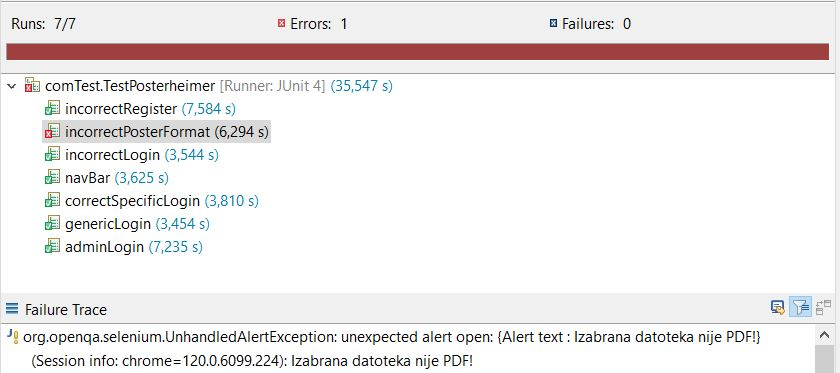
\includegraphics[width=\linewidth]{Slike/testResults}
				\caption{Prikaz uspješnosti ispitnih slučajeva}
			\end{figure}
			
			U \textbf{prvom ispitnom slučaju} provjerena je funkcionalnost gumba za pristup konferenciji pri incijalnom pristupu pomoću točnog generičkog korisničkog imena (email adrese predviđenu za generički račun) i odgovarajuće lozinke. Predviđen rezultat je dozvoljen pristup stranici konferencije. Ispitni slučaj je uspješan.
			
			
			\begin{lstlisting}
@Test
public void genericLogin() {
	
	System.setProperty("webdriver.chrome.driver", "C:\\Program Files (x86)\\Chrome Driver\\chromedriver.exe");
	WebDriver driver = new ChromeDriver();
	driver.manage().timeouts().implicitlyWait(10, TimeUnit.SECONDS);
	
	driver.get("https://posterheimer.onrender.com/");
	org.openqa.selenium.Dimension target = new  org.openqa.selenium.Dimension(1552, 840);
	driver.manage().window().setSize(target);
	
	driver.findElement(By.xpath("(//button[contains(text(),'Pristupi')])[4]")).click();
	// broj postaviti na mjesto konferencije u listi
	{
		WebElement element = driver.findElement(By.xpath("(//button[@type=\'button\'])[4]"));
		Actions builder = new Actions(driver);
		builder.moveToElement(element).perform();
	}
	{
		WebElement element = driver.findElement(By.tagName("body"));
		Actions builder = new Actions(driver);
		builder.moveToElement(element, 0, 0).perform();
	}
	
	driver.findElement(By.id("username")).click();
	driver.findElement(By.id("username")).sendKeys("visitor.test@mail.hr");
	driver.findElement(By.id("password")).click();
	driver.findElement(By.id("password")).sendKeys("pass");
	driver.findElement(By.cssSelector(".btn-primary")).click();
	
	driver.findElement(By.linkText("Konferencija")).click();
	
	String redirURL = driver.getCurrentUrl();
	boolean comperRes = redirURL.contains("/conference");
	if(comperRes == true) {
		System.out.println("Pristupljeno konferenciji");
	} else {
		System.out.println("Error");
	}
	assertEquals(comperRes, true);
	driver.quit();
}
			\end{lstlisting}
			
			U \textbf{drugom ispitnom slučaju} provjerena je funkcionalnost gumba za pristup konferenciji pomoću jedinstvenog korisničkog računa te odjava. Potrebno je upisati točnu email adresu i odgovarajuću lozinku već stvorenog korisničkog računa. Nakon upisa podataka, korisnik dobiva pristup stranici konferencije. Nakon prijave, korisnik se odjavljuje. Predviđen rezultat je povratak na početnu stranicu aplikacije. Ispitni slučaj je uspješan.  

			
			\begin{lstlisting}
@Test
public void correctSpecificLogin() {
	System.setProperty("webdriver.chrome.driver", "C:\\Program Files (x86)\\Chrome Driver\\chromedriver.exe");
	WebDriver driver = new ChromeDriver();
	driver.manage().timeouts().implicitlyWait(10, TimeUnit.SECONDS);
	
	driver.get("https://posterheimer.onrender.com/");
	driver.manage().window().setSize(new Dimension(1552, 840));
	driver.findElement(By.cssSelector(".list-group-item:nth-child(4) > .float-end")).click();
	driver.findElement(By.id("username")).click();
	driver.findElement(By.id("username")).sendKeys("register.email@mail.hr");
	driver.findElement(By.id("password")).click();
	driver.findElement(By.id("password")).sendKeys("pass");
	driver.findElement(By.cssSelector(".btn-primary")).click();
	
	driver.findElement(By.linkText("Konferencija")).click();
	
	String redirURL = driver.getCurrentUrl();
	boolean comperRes = redirURL.contains("/conference");
	if(comperRes == true) {
		System.out.println("Pristupljeno konferenciji");
	} else {
		System.out.println("Error: prijava");
	}
	
	driver.findElement(By.id("user-dropdown")).click();
	driver.findElement(By.cssSelector(".fa-right-from-bracket")).click();
	
	redirURL = driver.getCurrentUrl();
	comperRes = redirURL.equals("https://posterheimer.onrender.com/");
	if(comperRes == true) {
		System.out.println("Ostvarena odjava");
	} else {
		System.out.println("Error: odjava");
	}
	driver.quit();
}	
			\end{lstlisting}
			
			
			U \textbf{trećem ispitnom slučaju} provjerena je funkcionalnost gumba za pristup konferenciji pri neispravnoj prijavi. Predviđen rezultat je prikaz obavijesti "Pogrešan email ili lozinka!" te ostajanje na sučelju za prijavu unutar početne stranice. Ispitni slučaj je uspješan.
			
			\begin{lstlisting}
@Test
public void incorrectLogin() {
	System.setProperty("webdriver.chrome.driver", "C:\\Program Files (x86)\\Chrome Driver\\chromedriver.exe");
	WebDriver driver = new ChromeDriver();
	driver.manage().timeouts().implicitlyWait(10, TimeUnit.SECONDS);
	
	driver.get("https://posterheimer.onrender.com/");
	driver.manage().window().setSize(new Dimension(1552, 840));
	driver.findElement(By.xpath("(//button[@type=\'button\'])[3]")).click();
	{
		WebElement element = driver.findElement(By.xpath("(//button[@type=\'button\'])[3]"));
		Actions builder = new Actions(driver);
		builder.moveToElement(element).perform();
	}
	{
		WebElement element = driver.findElement(By.tagName("body"));
		Actions builder = new Actions(driver);
		builder.moveToElement(element, 0, 0).perform();
	}
	driver.findElement(By.cssSelector(".mb-3:nth-child(1)")).click();
	driver.findElement(By.id("username")).click();
	driver.findElement(By.id("username")).sendKeys("test");
	driver.findElement(By.id("password")).click();
	driver.findElement(By.id("password")).sendKeys("test");
	driver.findElement(By.cssSelector(".btn-primary")).click();
	
	driver.findElement(By.cssSelector(".alert")).click();
	{
		WebElement element = driver.findElement(By.cssSelector(".alert"));
		Actions builder = new Actions(driver);
		builder.doubleClick(element).perform();
	}
	WebElement alert = driver.findElement(By.cssSelector(".alert"));
	String errorMessage = alert.getText();
	if(errorMessage.contains("email ili lozinka!")) {
		System.out.println("Prikaz prikladne obavijesti");
	}
	
	driver.findElement(By.cssSelector(".btn-close")).click();
	
	String redirURL = driver.getCurrentUrl();
	boolean comperRes = redirURL.equals("https://posterheimer.onrender.com/");
	if(comperRes) {
		System.out.println("Ostvaren rezultat");
	}
	driver.quit();
}
			\end{lstlisting}
			
			U \textbf{četvrtom ispitnom slučaju} provjerena je funkcionalnost gumba za pristup konferenciji pri prijavi administratora. Predviđen rezultat je dozvoljen pristup konferenciji te mogućnost dodavanja postera, fotografija i pokrovitelja. Ispitni slučaj je uspješan.
			
			\begin{lstlisting}
	  @Test
public void adminLogin() {
	System.setProperty("webdriver.chrome.driver", "C:\\Program Files (x86)\\Chrome Driver\\chromedriver.exe");
	WebDriver driver = new ChromeDriver();
	driver.manage().timeouts().implicitlyWait(20, TimeUnit.SECONDS);
	// Vrijeme povecano zbog ucitavanja postera, koje je znatno sporije za administratora
	
	driver.get("https://posterheimer.onrender.com/");
	driver.manage().window().setSize(new Dimension(1552, 840));
	driver.findElement(By.cssSelector(".list-group-item:nth-child(3) > .float-end")).click();
	driver.findElement(By.id("username")).click();
	driver.findElement(By.id("username")).sendKeys("admin.test@mail.hr");
	driver.findElement(By.id("password")).click();
	driver.findElement(By.id("password")).sendKeys("pass");
	driver.findElement(By.cssSelector(".btn-primary")).click();
	driver.findElement(By.cssSelector(".conference-content")).click();
	driver.findElement(By.linkText("Posteri")).click();
	driver.findElement(By.cssSelector(".fa-solid")).click();
	driver.findElement(By.cssSelector(".btn-close")).click();
	driver.findElement(By.linkText("Fotografije")).click();
	driver.findElement(By.cssSelector(".image-container > img")).click();
	driver.findElement(By.cssSelector(".modal-title")).click();
	driver.findElement(By.cssSelector(".modal-title")).click();
	{
		WebElement element = driver.findElement(By.cssSelector(".modal-title"));
		Actions builder = new Actions(driver);
		builder.doubleClick(element).perform();
	}
	driver.findElement(By.cssSelector(".modal-title")).click();
	driver.findElement(By.cssSelector(".modal-title")).click();
	driver.findElement(By.cssSelector(".btn-close")).click();
	driver.findElement(By.linkText("Pokrovitelji")).click();
	driver.findElement(By.cssSelector(".fa-solid")).click();
	driver.findElement(By.cssSelector(".modal-title")).click();
	driver.findElement(By.cssSelector(".btn-close")).click();
	
	String redirURL = driver.getCurrentUrl();
	boolean comperRes = redirURL.contains("sponsors");
	if(comperRes) {
		System.out.println("Ostvaren rezultat");
	}
	driver.quit();
}
			\end{lstlisting}
			
			
	U \textbf{petom ispitnom slučaju} provjerena je funkcionalnost navigacijske trake. Predviđen rezultat je otvaranje stranice konferencije nakon klika na "Konferencija", stranice postera nakon klika na "Posteri", stranice za fotografije nakon klika na "Fotografije" i stranice pokrovitelja nakon klika na "Pokrovitelji". Ispitni slučaj je uspješan.
	
	\begin{lstlisting}
	  @Test
public void navBar() {
	System.setProperty("webdriver.chrome.driver", "C:\\Program Files (x86)\\Chrome Driver\\chromedriver.exe");
	WebDriver driver = new ChromeDriver();
	driver.manage().timeouts().implicitlyWait(10, TimeUnit.SECONDS);	
	
	driver.get("https://posterheimer.onrender.com/");
	org.openqa.selenium.Dimension target = new  org.openqa.selenium.Dimension(1552, 840);
	driver.manage().window().setSize(target);
	
	driver.findElement(By.xpath("(//button[contains(text(),'Pristupi')])[3]")).click();
	// broj postaviti na mjesto konferencije u listi
	{
		WebElement element = driver.findElement(By.xpath("(//button[@type=\'button\'])[3]"));
		Actions builder = new Actions(driver);
		builder.moveToElement(element).perform();
	}
	{
		WebElement element = driver.findElement(By.tagName("body"));
		Actions builder = new Actions(driver);
		builder.moveToElement(element, 0, 0).perform();
	}
	
	driver.findElement(By.id("username")).click();
	driver.findElement(By.id("username")).sendKeys("visitor.test@mail.hr");
	driver.findElement(By.id("password")).click();
	driver.findElement(By.id("password")).sendKeys("pass");
	driver.findElement(By.cssSelector(".btn-primary")).click();
	
	driver.findElement(By.linkText("Konferencija")).click();
	String redirURL = driver.getCurrentUrl();
	boolean comperRes = redirURL.contains("/conference");
	if(comperRes == true) {
		System.out.println("Pristupljeno konferenciji");
	} else {
		System.out.println("Error: konferencije");
	}
	
	driver.findElement(By.linkText("Posteri")).click();
	redirURL = driver.getCurrentUrl();
	comperRes = redirURL.contains("/posters");
	if(comperRes == true) {
		System.out.println("Pristupljeno posterima");
	} else {
		System.out.println("Error: posteri");
	}
	
	driver.findElement(By.linkText("Fotografije")).click();
	redirURL = driver.getCurrentUrl();
	comperRes = redirURL.contains("/photos");
	if(comperRes == true) {
		System.out.println("Pristupljeno fotografijama");
	} else {
		System.out.println("Error: fotografije");
	}
	driver.findElement(By.linkText("Pokrovitelji")).click();
	redirURL = driver.getCurrentUrl();
	comperRes = redirURL.contains("/sponsors");
	if(comperRes == true) {
		System.out.println("Pristupljeno pokroviteljima");
	} else {
		System.out.println("Error: pokrovitelji");
	}
	driver.quit();
}
	\end{lstlisting}
	
	U \textbf{šestom ispitnom slučaju} provjerena je funkcionalnost gumba za registraciju pri unosu email adrese netočnog formata. Predviđen rezultat je neuspješna registracija te obavijest o netočnom unosu. Ispitni slučaj je uspješan. 

			\begin{lstlisting}
	  @Test
public void incorrectRegister() {
	System.setProperty("webdriver.chrome.driver", "C:\\Program Files (x86)\\Chrome Driver\\chromedriver.exe");
	WebDriver driver = new ChromeDriver();
	JavascriptExecutor js = (JavascriptExecutor) driver;
	driver.manage().timeouts().implicitlyWait(10, TimeUnit.SECONDS);
	
	driver.get("https://posterheimer.onrender.com/");
	driver.manage().window().setSize(new Dimension(1552, 840));
	driver.findElement(By.cssSelector(".list-group-item:nth-child(3) > .float-end")).click();
	driver.findElement(By.cssSelector("form")).click();
	driver.findElement(By.id("username")).click();
	driver.findElement(By.id("username")).sendKeys("visitor.test@mail.hr");
	driver.findElement(By.id("password")).click();
	driver.findElement(By.id("password")).sendKeys("pass");
	driver.findElement(By.cssSelector(".btn-primary")).click();
	driver.findElement(By.linkText("Registracija")).click();
	js.executeScript("window.scrollTo(0,0)");
	driver.findElement(By.id("formIme")).click();
	driver.findElement(By.id("formIme")).sendKeys("TestIme");
	driver.findElement(By.id("formPrezime")).click();
	driver.findElement(By.id("formPrezime")).sendKeys("TestPrezime");
	driver.findElement(By.id("formBasicEmail")).click();
	driver.findElement(By.id("formBasicEmail")).sendKeys("email");
	driver.findElement(By.id("formBasicPassword")).click();
	driver.findElement(By.id("formBasicPassword")).sendKeys("lozinka");
	driver.findElement(By.cssSelector(".mb-3:nth-child(2) > #formBasicPassword")).click();
	driver.findElement(By.cssSelector(".mb-3:nth-child(2) > #formBasicPassword")).sendKeys("lozinka");
	driver.switchTo().frame(0);
	driver.findElement(By.cssSelector(".recaptcha-checkbox-border")).click();
	driver.switchTo().defaultContent();
	driver.findElement(By.cssSelector(".ml-2")).click();
	driver.findElement(By.cssSelector(".mx-2 > .mb-3:nth-child(1)")).click();
	driver.findElement(By.cssSelector(".mx-2 > .mb-3:nth-child(1)")).click();
	{
		WebElement element = driver.findElement(By.cssSelector(".mx-2 > .mb-3:nth-child(1)"));
		Actions builder = new Actions(driver);
		builder.doubleClick(element).perform();
	}
	
	String redirURL = driver.getCurrentUrl();
	boolean comperRes = redirURL.contains("/register");
	if(comperRes == true) {
		System.out.println("Neuspjesna registracija");
	} else {
		System.out.println("Error");
	}
	
	driver.quit();
}	  
			\end{lstlisting}
			
			
			\subsection{Ispitivanje sustava}
			
			 \textit{Potrebno je provesti i opisati ispitivanje sustava koristeći radni okvir Selenium\footnote{\url{https://www.seleniumhq.org/}}. Razraditi \textbf{minimalno 4 ispitna slučaja} u kojima će se ispitati redovni slučajevi, rubni uvjeti te poziv funkcionalnosti koja nije implementirana/izaziva pogrešku kako bi se vidjelo na koji način sustav reagira kada nešto nije u potpunosti ostvareno. Ispitni slučaj se treba sastojati od ulaza (npr. korisničko ime i lozinka), očekivanog izlaza ili rezultata, koraka ispitivanja i dobivenog izlaza ili rezultata.\\ }
			 
			 \textit{Izradu ispitnih slučajeva pomoću radnog okvira Selenium moguće je provesti pomoću jednog od sljedeća dva alata:}
			 \begin{itemize}
			 	\item \textit{dodatak za preglednik \textbf{Selenium IDE} - snimanje korisnikovih akcija radi automatskog ponavljanja ispita	}
			 	\item \textit{\textbf{Selenium WebDriver} - podrška za pisanje ispita u jezicima Java, C\#, PHP koristeći posebno programsko sučelje.}
			 \end{itemize}
		 	\textit{Detalji o korištenju alata Selenium bit će prikazani na posebnom predavanju tijekom semestra.}
		 	
		 	Ispitivanje sustava provedeno je pomoću dodatka za preglednik Selenium IDE\footnote{https://www.selenium.dev/selenium-ide/}.
		 	
		 	\textbf{Prvi ispitni slučaj} provjerava funkcionalnost brisanja korisnika. Prije brisanja korisnika potrebna je prijava registratora. Administrator briše određenog korisnika te se odjavljuje. Uspješnost brisanja korisnika provjeravamo pokušajem prijave izbrisanog korisnika. Očekivani rezultat je neuspješna prijava. Ispitni slučaj je uspješan.
		 	
		 	\begin{figure} [hbt!]
		 		\includegraphics[width=\linewidth]{Slike/deleteUser}
		 		\caption{Prikaz uspješnosti ispitnog slučaja}
		 	\end{figure}
		 	
		\begin{lstlisting}
  @Test
public void deleteUser() {
	driver.get("https://posterheimer.onrender.com/");
	driver.manage().window().setSize(new Dimension(1552, 840));
	driver.findElement(By.cssSelector(".list-group-item:nth-child(5) > .float-end")).click();
	{
		WebElement element = driver.findElement(By.cssSelector(".list-group-item:nth-child(5) > .float-end"));
		Actions builder = new Actions(driver);
		builder.moveToElement(element).perform();
	}
	{
		WebElement element = driver.findElement(By.tagName("body"));
		Actions builder = new Actions(driver);
		builder.moveToElement(element, 0, 0).perform();
	}
	driver.findElement(By.cssSelector(".mb-3:nth-child(1)")).click();
	driver.findElement(By.id("username")).click();
	driver.findElement(By.id("username")).sendKeys("admin.test@mail.hr");
	driver.findElement(By.cssSelector("form")).click();
	driver.findElement(By.id("password")).click();
	driver.findElement(By.id("password")).sendKeys("pass");
	driver.findElement(By.cssSelector(".btn-primary")).click();
	driver.findElement(By.id("user-dropdown")).click();
	driver.findElement(By.linkText("Korisnici")).click();
	driver.findElement(By.cssSelector(".list-group-item:nth-child(16) > .float-start")).click();
	driver.findElement(By.id("root")).click();
	driver.findElement(By.cssSelector(".list-group-item:nth-child(18) > .btn")).click();
	driver.findElement(By.id("user-dropdown")).click();
	driver.findElement(By.linkText("Odjava")).click();
	driver.findElement(By.cssSelector(".list-group-item:nth-child(5) > .float-end")).click();
	{
		WebElement element = driver.findElement(By.cssSelector(".list-group-item:nth-child(5) > .float-end"));
		Actions builder = new Actions(driver);
		builder.moveToElement(element).perform();
	}
	{
		WebElement element = driver.findElement(By.tagName("body"));
		Actions builder = new Actions(driver);
		builder.moveToElement(element, 0, 0).perform();
	}
	driver.findElement(By.id("username")).click();
	driver.findElement(By.id("username")).sendKeys("register2.");
	driver.findElement(By.id("username")).sendKeys("register2.email@mail.hr");
	driver.findElement(By.id("password")).click();
	driver.findElement(By.id("password")).sendKeys("pass");
	driver.findElement(By.cssSelector(".btn-primary")).click();
}
		\end{lstlisting}
		
\textbf{Drugi ispitni slučaj} provjerava funkcionalnost gumba za registraciju pri unosu podataka točnog formata. Tijekom registracije odabrana je opcija "Prikaz lozinke" te prođen CAPTCHA test. Rezultat ispitnog slučaja je uspješan.

\begin{figure} [hbt!]
	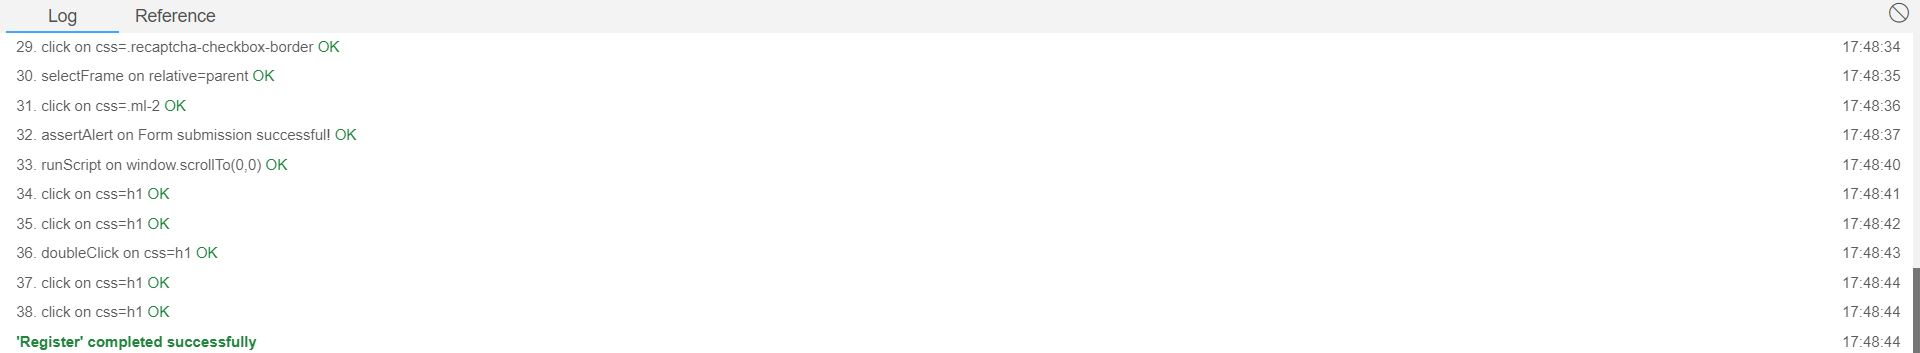
\includegraphics[width=\linewidth]{Slike/Register}
	\caption{Prikaz uspješnosti ispitnog slučaja}
\end{figure}

\begin{lstlisting}
	@Test
	public void register() {
		driver.get("https://posterheimer.onrender.com/");
		driver.manage().window().setSize(new Dimension(1552, 840));
		driver.findElement(By.cssSelector(".list-group-item:nth-child(5) > .float-end")).click();
		driver.findElement(By.id("username")).click();
		driver.findElement(By.id("username")).sendKeys("visitor.test@mail.hr");
		driver.findElement(By.id("password")).click();
		driver.findElement(By.id("password")).sendKeys("pass");
		driver.findElement(By.cssSelector(".btn-primary")).click();
		driver.findElement(By.cssSelector(".conference-content")).click();
		driver.findElement(By.cssSelector(".mx-auto:nth-child(1)")).click();
		driver.findElement(By.cssSelector(".card-text")).click();
		driver.findElement(By.linkText("Registracija")).click();
		js.executeScript("window.scrollTo(0,0)");
		driver.findElement(By.id("formIme")).click();
		driver.findElement(By.id("formIme")).sendKeys("TestIme");
		driver.findElement(By.id("formPrezime")).click();
		driver.findElement(By.id("formPrezime")).sendKeys("TestPrezime");
		driver.findElement(By.id("formBasicEmail")).click();
		driver.findElement(By.id("formBasicEmail")).click();
		driver.findElement(By.id("formBasicEmail")).sendKeys("register.email@mail.hr"); // promijeniti email za svaki test
		driver.findElement(By.id("formBasicPassword")).click();
		driver.findElement(By.id("formBasicPassword")).sendKeys("pass");
		driver.findElement(By.cssSelector(".mb-3:nth-child(2) > #formBasicPassword")).click();
		driver.findElement(By.cssSelector(".mb-3:nth-child(2) > #formBasicPassword")).sendKeys("pass");
		driver.findElement(By.cssSelector(".form-check")).click();
		driver.findElement(By.id("formShowPassword")).click();
		driver.findElement(By.id("formShowPassword")).click();
		driver.switchTo().frame(0);
		driver.findElement(By.cssSelector(".recaptcha-checkbox-border")).click();
		driver.switchTo().defaultContent();
		driver.findElement(By.cssSelector(".ml-2")).click();
		assertThat(driver.switchTo().alert().getText(), is("Form submission successful!"));
		js.executeScript("window.scrollTo(0,0)");
		driver.findElement(By.cssSelector("h1")).click();
		driver.findElement(By.cssSelector("h1")).click();
		{
			WebElement element = driver.findElement(By.cssSelector("h1"));
			Actions builder = new Actions(driver);
			builder.doubleClick(element).perform();
		}
		driver.findElement(By.cssSelector("h1")).click();
		driver.findElement(By.cssSelector("h1")).click();
	}
\end{lstlisting}

\textbf{Treći ispitni slučaj} provjerava funkcionalnost gumba za dodavanje konferencije. Prije dodavanja konferencije potrebna je prijava natkorisnika. Podaci vezani za korisnički račun natkorisnika uklonjeni su iz izvornog koda. Predviđen rezultat  je stvaranje nove konferencije. Ispitni slučaj je uspješan.

\begin{figure} [hbt!]
	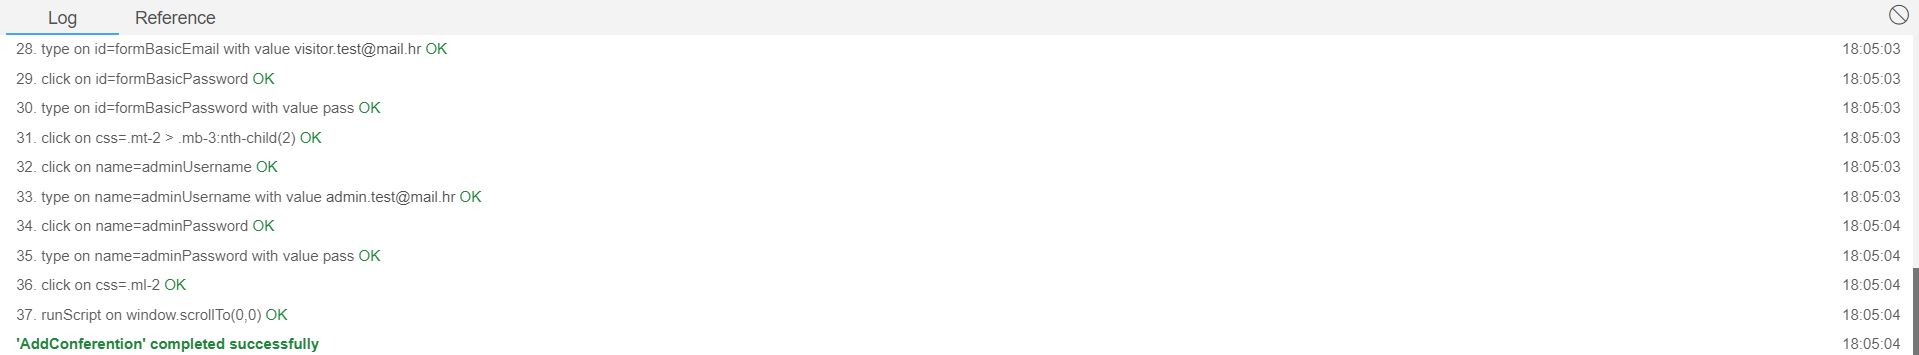
\includegraphics[width=\linewidth]{Slike/addConferention}
	\caption{Prikaz uspješnosti ispitnog slučaja}
\end{figure}

\begin{lstlisting}
	@Test
	public void addConferention() {
		driver.get("https://posterheimer.onrender.com/");
		driver.manage().window().setSize(new Dimension(1552, 840));
		driver.findElement(By.cssSelector(".fa-solid")).click();
		driver.findElement(By.id("username")).click();
		driver.findElement(By.id("username")).sendKeys("ime natkorisnika");
		driver.findElement(By.id("password")).click();
		driver.findElement(By.id("password")).sendKeys("lozinka natkorisnika");
		driver.findElement(By.cssSelector(".btn-primary")).click();
		driver.findElement(By.cssSelector(".fa-square-plus")).click();
		driver.findElement(By.id("formConferenceName")).click();
		driver.findElement(By.id("formConferenceName")).sendKeys("AutomaticTestKonferencija");
		driver.findElement(By.name("videoUrl")).click();
		driver.findElement(By.name("videoUrl")).sendKeys("https://www.youtube.com/watch?v=ScMzIvxBSi4&ab_channel=BenMarquezTX");
		driver.findElement(By.id("formConferenceCity")).click();
		driver.findElement(By.id("formConferenceCity")).sendKeys("Unska ");
		driver.findElement(By.id("formConferenceCity")).sendKeys("Unska 3");
		driver.findElement(By.id("formConferenceLocation")).click();
		driver.findElement(By.id("formConferenceLocation")).sendKeys("Zagreb");
		driver.findElement(By.id("formConferenceZipCode")).click();
		driver.findElement(By.id("formConferenceZipCode")).sendKeys("10000");
		driver.findElement(By.id("formDateStart")).click();
		driver.findElement(By.id("formDateStart")).sendKeys("2024-01-11T09:13");
		driver.findElement(By.id("formDateEnd")).click();
		driver.findElement(By.id("formDateEnd")).sendKeys("2024-01-14T09:13");
		driver.findElement(By.id("root")).click();
		driver.findElement(By.id("formBasicEmail")).click();
		driver.findElement(By.id("formBasicEmail")).sendKeys("visitor");
		driver.findElement(By.id("formBasicEmail")).sendKeys("visitor.test@mail.hr");
		driver.findElement(By.id("formBasicPassword")).click();
		driver.findElement(By.id("formBasicPassword")).sendKeys("pass");
		driver.findElement(By.cssSelector(".mt-2 > .mb-3:nth-child(2)")).click();
		driver.findElement(By.name("adminUsername")).click();
		driver.findElement(By.name("adminUsername")).sendKeys("admin.test@mail.hr");
		driver.findElement(By.name("adminPassword")).click();
		driver.findElement(By.name("adminPassword")).sendKeys("pass");
		driver.findElement(By.cssSelector(".ml-2")).click();
		js.executeScript("window.scrollTo(0,0)");
	}
\end{lstlisting}
		 	
		 	
		\textbf{Četvrti ispitni slučaj:} prijava registriranog korisnika, odlazak na postere, glasanje za jedan od postera, pokušaj glasanja za drugi poster. Očekivani rezultat je obavijest koja korisniku govori da je nemoguće glasati više od jedanput
			
			\eject 
		
		
		\section{Dijagram razmještaja}
			
			\textbf{\textit{dio 2. revizije}}
			
			 \textit{Potrebno je umetnuti \textbf{specifikacijski} dijagram razmještaja i opisati ga. Moguće je umjesto specifikacijskog dijagrama razmještaja umetnuti dijagram razmještaja instanci, pod uvjetom da taj dijagram bolje opisuje neki važniji dio sustava.}
			 
			 \indent Dijagram razmještaja prikazuje odnos sklopovskih dijelova sustava međusobno i s programskim rješenjima koja su potrebna za korisnikovu interakciju s aplikacijom. Kao dio udaljene poslužiteljske infrastrukture postoje dva poslužiteljska računala: mrežni poslužitelj i poslužitelj baze podataka. Na mrežnom poslužitelju je aktivan proces programa aplikacije koji komunicira s bazom podataka koja je aktivna na vlastitom poslužitelju. Predviđeno je da korisnik koristi mrežni preglednik na vlastitom računalu za komunikaciju s aplikacijom na mrežnom poslužitelju.
			 
			 \begin{figure} [hbt!]
			 	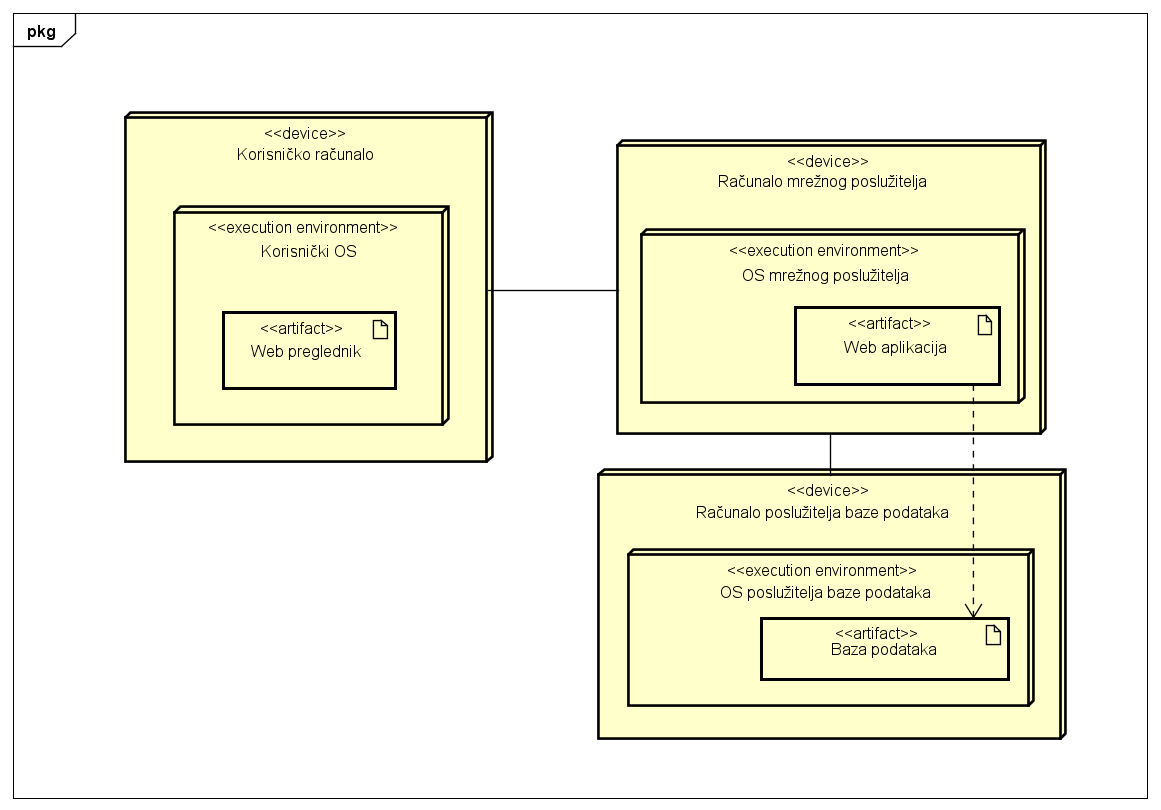
\includegraphics[width=\linewidth]{Slike/DeploymentDiagram}
			 	\caption{Dijagram razmještaja}
			 \end{figure}
			
			\eject 
		
		\section{Upute za puštanje u pogon}
		
			\textbf{\textit{dio 2. revizije}}\\
		
			 \textit{U ovom poglavlju potrebno je dati upute za puštanje u pogon (engl. deployment) ostvarene aplikacije. Na primjer, za web aplikacije, opisati postupak kojim se od izvornog kôda dolazi do potpuno postavljene baze podataka i poslužitelja koji odgovara na upite korisnika. Za mobilnu aplikaciju, postupak kojim se aplikacija izgradi, te postavi na neku od trgovina. Za stolnu (engl. desktop) aplikaciju, postupak kojim se aplikacija instalira na računalo. Ukoliko mobilne i stolne aplikacije komuniciraju s poslužiteljem i/ili bazom podataka, opisati i postupak njihovog postavljanja. Pri izradi uputa preporučuje se \textbf{naglasiti korake instalacije uporabom natuknica} te koristiti što je više moguće \textbf{slike ekrana} (engl. screenshots) kako bi upute bile jasne i jednostavne za slijediti.}
			
			
			 \textit{Dovršenu aplikaciju potrebno je pokrenuti na javno dostupnom poslužitelju. Studentima se preporuča korištenje neke od sljedećih besplatnih usluga: \href{https://aws.amazon.com/}{Amazon AWS}, \href{https://azure.microsoft.com/en-us/}{Microsoft Azure} ili \href{https://www.heroku.com/}{Heroku}. Mobilne aplikacije trebaju biti objavljene na F-Droid, Google Play ili Amazon App trgovini.}
			
			
			\eject 